Um die Funktion des Lock-In-Verstärkers kennenzulernen, stehen ein modular
aufgebauter Verstärker (Abbildung \ref{fig:verstärker}) und ein
Speicher-Oszilloskop zur Verfügung.
\begin{figure}[h]
  \centering
  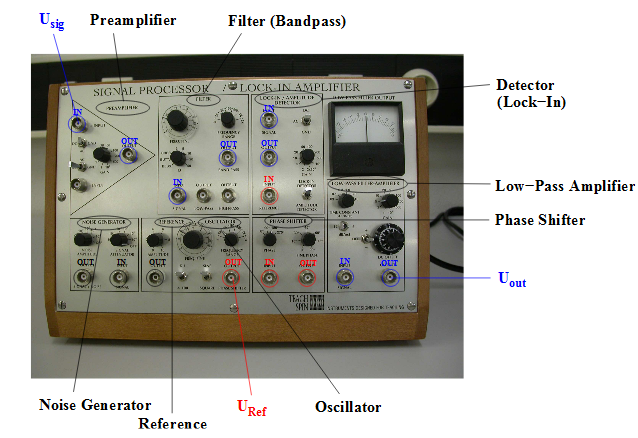
\includegraphics[height=7.5cm]{Bilder/Verstaerker.jpg}
  \caption{Verstärker \;\cite{303}}
  \label{fig:verstärker}
\end{figure}
\\
Ein Lock-In-Verstärker besteht in der Regel aus folgenden Bauteilen:
\begin{itemize}
  \item Vorverstärker
  \item Hoch-, Tief- und Bandpassfilter
  \item Phasenverschieber für die Anpassung zwischen Referenz- und Messignal
  \item Funktionsgenerator
%  \item Rauschgenerator
  \item Tiefpass-Verstärker
  \item Amplituden/Lock-In-Detektor
\end{itemize}
Die Signale der einzelnen Komponenten können über das verwendete
Speicher-Oszilloskop seperat betrachtet und vermessen werden.
\newpage
In einem ersten Schritt wird die Schaltung aus Abbildung \ref{fig:schalt}
aufgebaut.
\begin{figure}[h]
  \centering
  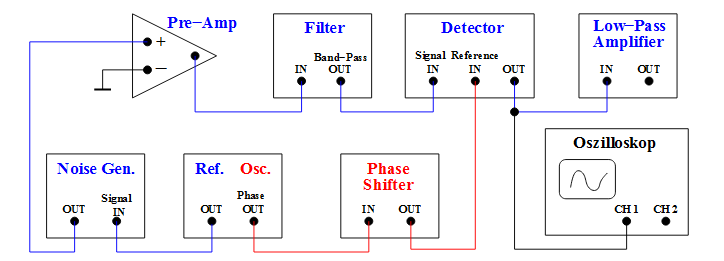
\includegraphics[width=\textwidth]{Bilder/Schaltung.jpg}
  \caption{Schaltbild Lock-In-Verstärker \;\cite{303}}
  \label{fig:schalt}
\end{figure}
\\
Hierbei wird nach jedem Bauteil überprüft, welche Signalformen ausgegeben werden.
Für den ersten Teil des Versuchs wird der Noise-Generator zunächst überbrückt.
Das Eingangssignal $U_\text{sig}$ wird nun auf eine Frequenz von $1\;\si{\kilo\hertz}$
und eine Spannung von $10\;\si{\milli\volt}$ eingestellt. Dieses Signal wird dann
auf den Verstärker gegeben und am Ausgang mit einem sinusförmigen Signal gleicher
Frequenz gemischt. Mit diesen Einstellungen werden Ausgangssignale für 5 verschiedene
Phasen skizziert.
Nachdem die Ausgangssignale skizziert wurden, wird der Tiefpass hinzugeschaltet
und die Abhängigkeit des Ausgangsstroms zur Phasenverschiebung
$\Delta\varphi$ gemessen.
% klingt noch ziemlich komisch
Danach werden die Messungen mit zugeschaltenem Rausch-Generator wiederholt. Das Signal
kann an verschiedenen Stellen verstärkt werden, z.B. an den Filtern, dem Oszilloskop
oder am Pre-Amplifier.
\\
\begin{figure}
  \centering
  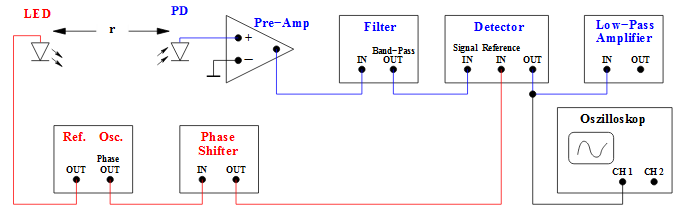
\includegraphics[width=\textwidth]{Bilder/LEDSchaltung.jpg}
  \caption{Schaltung mit Leuchtdiode \cite{303}}
  \label{fig:LED}
\end{figure}  % Hier evtl Bild und Text tauschen
\\
Im zweiten Teil des Experiments wird die Schaltung wie in Abbildung \ref{fig:LED}
aufgebaut. Die Frequenz der LED liegt hierbei zwischen $100 \;\si{\hertz}$ und
$300 \;\si{\hertz}$.
Die Photodiode (PD) misst das aussgesendete Licht.
Damit soll die Lichtintensität der LED in Abhängigkeit des Abstands
zwischen LED und PD gemessen werden. Zudem soll überprüft werden, bis zu welchem
Abstand $r_\text{max}$ das Licht der LED nachgewiesen werden kann. Hierfür
ist die LED fest am Ende einer Schiene und die PD beweglich auf ihr montiert.
Anhand einer Skala, auf der Schiene, wird der Abstand der PD abgelesen.
\newpage
